\cotefile{71}
\scanpage{28}
\figure{%
\begin{tikzpicture}[x=0.016cm,y=0.016cm,line cap=round,line join=round]
  \draw[line width=1.1pt] (0,0) -- (55,49) -- (91,85);
  \draw[line width=.45pt]
    (55,49) -- (58,68)
    (58,77) .. controls (59,88) and (60,106) .. (62,116)
    (62,116) -- (67,140)
    (71,157) -- (77,179)
    (79,193) -- (81,207);
  \draw[line width=.2pt] (59,90) .. controls (63,94) and (65,102) .. (64,106);
  \foreach \point in {(0,0),(55,49),(91,85),(84,216)}
    \fill \point circle[radius=1.2pt];
  \node[above right,inner sep=1pt] at (84,216) {$x$};
  \node[left,inner sep=2pt] at (55,51) {$y$};
  \node[below left,inner sep=1pt] at (0,0) {$\unsure{s|z}$};
  \node[right,inner sep=2pt] at (91,85) {$s'$};
\end{tikzpicture}}
% archive sheet number: 27
\scanpage{29}\mspage{V}
\deleted{$]z,x]\subset\mathbb{R}^{2}-\mathbb{C}$, c.q.f.d.}

% slanted
\margin{\uline{\unsure{visa}}}
\uline{Lemme} V. Soit $\mathbb{C}$ un \uline{ensemble convexe} nonvide de $\mathbb{R}^{2}$ et soit $y\in\mathbb{C}$ tel qu'il existe $s,s'\in\mathbb{C}$ avec $y\in ]s,s'[$. Supposons que $y$ est $(\mathbb{R}^{2}-C)$-visible d'un point $x\notin\mathbb{C}$ qui n'est pas colineaire avec $s$ et $s'$. Alors tout point colineaire avec $s$ et $s'$ est \inserted{$(\mathbb{R}^{2}-\mathbb{C})$-}visible de $x$.

\margin{\uline{NB} $s,s'$ \unsure{appartiennent} à une \unsure{même} \unsure{arête} de $C$, et si $D$ est la droite qu'elle \unsure{détermine} $x$ et $C$ sont de part et d'autre de cette droite\ldots}

\uline{Demonstration} : Soit $d$ la droite determinée par $s$ et par $s'$, et appelons $\mathbb{S}_{1}$ et $\mathbb{S}_{2}$ les deux demi-espaces ouverts dans lesquels $\mathbb{R}^{2}$ est partagé par $d$.

Comme $x$ n'est pas colineaire avec $s$ et $s'$, \deleted{\unsure{ou|on}} $x\in S_{1}$ ou bien $x\in S_{2}$.

Supposons que $x\in\mathbb{S}_{1}$ et $z\in d$ et prouvons que $]x,z[\subset\mathbb{R}^{2}-\mathbb{C}$. Si $]x,z[\not\subset\mathbb{R}^{2}\deleted{\unsure{,}}-\mathbb{C}$ il doit exister $w\in ]x,z[\cap\mathbb{C}{}^{\inserted{\subset\mathbb{S}_{1}}}$. Comme $w\in\mathbb{S}_{1}$ aussi, les trois points $s_{\deleted{\unsure{1}}},s_{\deleted{\unsure{2}}}',w$ sont affinement independants.

Considerons donc le triangle $T$ de sommets $s,s',w$ (i.e. l'enveloppe convexe de $\{s',s,w\}$). Comme $[x,\deleted{\unsure{z}}y]\cap ]s,s'[\ne\varnothing$ on a aussi $[x,y\deleted{\unsure{]}}[\cap T\ne\varnothing$, mais $T\subset\mathbb{C}$ puisque $\{s,s',w\}\subset\mathbb{C}$ ce qui est un \unsure{absurd} \inserted{puisque on suppose $[x,y[\cap\mathbb{C}=\varnothing$}, cela prouve donc le lemme.

% A short bent pen stroke in the left margin faces the heading.
\margin{\tikz[baseline]{\draw[line cap=round] (0,0) .. controls (-.02,.16) and (0,.21) .. (.08,.23) -- (.34,.36);}}
\uline{Definition} 3. Un polygone $\Gamma$ est \inserted{dit} convexe \inserted{(par abus de \unsure{langage} !)} si l'ensemble sous-jacent à $\Gamma$ est le bord d'un ensemb\uline{le} \uline{co}nvexe (i.e. $\Gamma=\mathbb{C}-\mathring{\mathbb{C}}$, $\mathbb{C}$ convexe)

On peut maintenant én\deleted{\unsure{n}}oncer le :

\uline{Lemme} VI. Si $\Gamma$ est un polygone convexe alors $\Gamma$ est un J-polygone et tout sommet de $\Gamma$ \deleted{\illegible{1}} qui n'est pas colinéaire avec \deleted{\unsure{s}}les deux sommets adjacents ($=$ consecutifs) est un bon sommet (cf. def.2)
% archive sheet number: 28
\scanpage{30}
% margin note written sideways
\margin{\deleted{alors [les \unsure{comp.} connexes de $\Gamma\cap[s',s'']$ sont des \inserted{côtés et des} segments \unsure{$I_{\alpha}$}, des points \inserted{sommets de \deleted{\unsure{$\Gamma$}}$S$}, et les extrémités des $\unsure{I_{\alpha}}$ et] les \unsure{sg. de} $\unsure{*}$} $S(\Gamma)\cap ]s',s''[\ne\unsure{\varnothing|\psi}$, \deleted{et que, soit $t\in$} alors $\unsure{\mathcal{L}|\mathscr{L}|L}=S(\Gamma)\cap\unsure{(}T-\{s,s',s''\}\unsure{\}|\!)}\deleted{\unsure{[s',s''])}},\ne\varnothing$, et $t\in\mathcal{L}$ \unsure{réalise} le maximum de la distance à la droite définie par $s',s''$, alors $]s,t[\subset\operatorname{Int}\Gamma$.}
% margin note written sideways
\margin{\uline{Corollaire} Ou bien $]s',s''[\subset\operatorname{Int}\Gamma$, ou bien $\exists\,t\in S(\Gamma)$, $t\ne\unsure{s}\unsure{\}|{}'}$, tel que $]s,t[\subset\operatorname{Int}\Gamma$.}

\figure{%
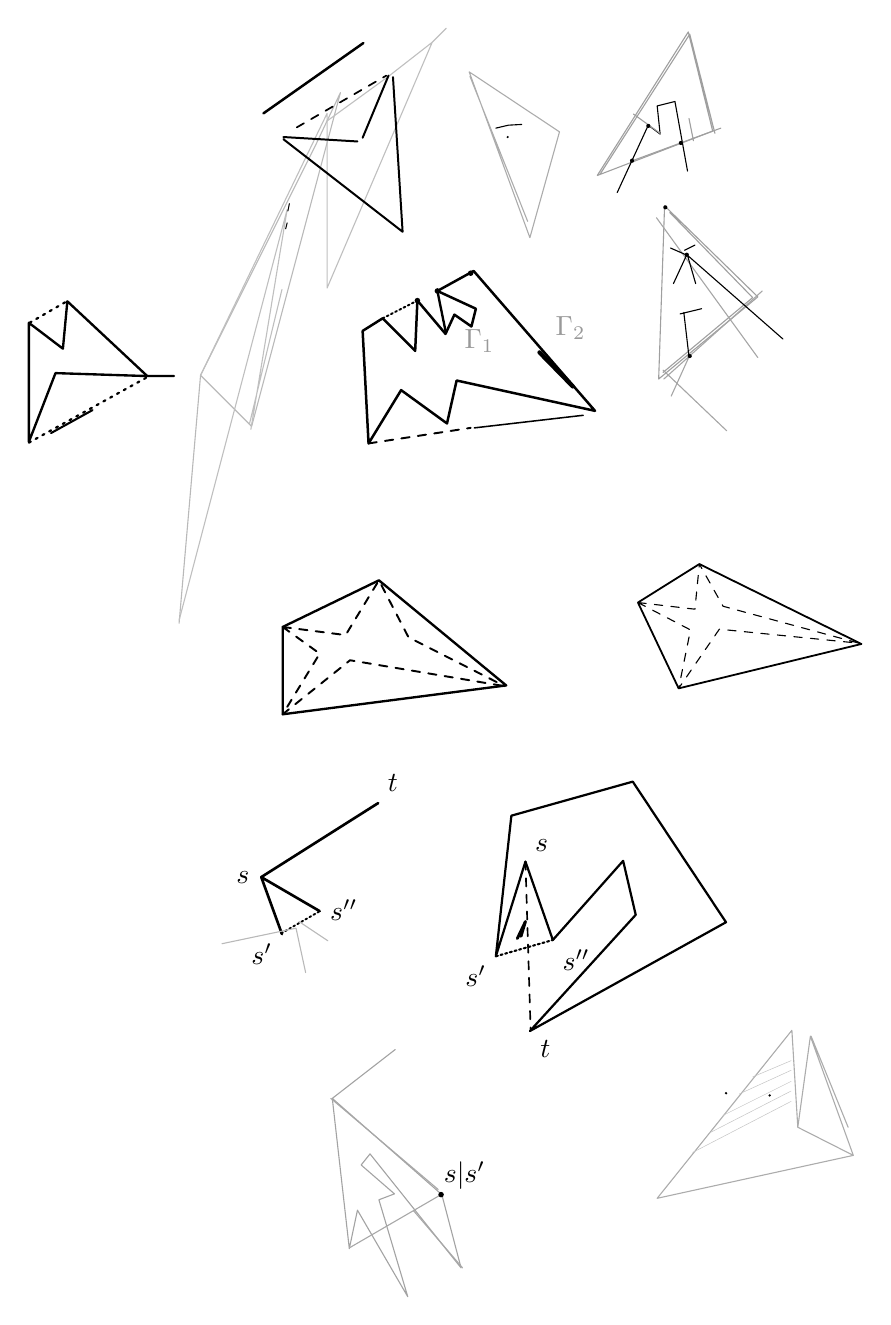
\begin{tikzpicture}[x=.0094cm,y=-.0094cm,line cap=round,line join=round]
% Pencil construction behind the dark reentrant triangle.
  \draw[gray!55] (586,906)--(615,571)--(770,261)--(804,189)--(684,640)--(615,571);
  \draw[gray!50] (586,902)--(732,347)--(683,644)
    (615,571)--(786,217)--(786,453)--(928,121)--(947,102)
    (785,228)--(869,167)--(928,121) (725,455)--(681,637);
  \draw[line width=.37pt] (735,339)--(733,349) (732,365)--(730,373);
  \draw[line width=.9pt] (700,217)--(835,122);
  \draw[line width=.72pt] (727,249)--(827,255) (834,250)--(869,166)
    (875,168)--(888,377)--(727,252);
  \draw[line width=.62pt,dashed] (745,236)--(866,166);
% Small pale triangle to the right.
  \draw[gray!65] (978,161)--(1100,242)--(1060,385)--cycle (979,167)--(1057,363);
  \draw (1014,237)--(1031,233)--(1049,232);
  \fill (1030,249) circle[radius=.43pt];
% Two upper-right pencil triangles and the strokes extended beyond their bases.
  \draw[gray!75] (1151,301)--(1274,107)--(1307,241)--cycle
    (1155,299)--(1276,110)--(1310,244);
  \draw (1178,324)--(1220,233)--(1236,245)--(1232,207)--(1256,201)--(1273,295);
  \draw[gray!75] (1200,218)--(1236,244) (1275,224)--(1281,254) (1196,282)--(1318,237);
  \foreach \p in {(1198,281),(1220,234),(1264,257)} \fill \p circle[radius=.75pt];
  \draw[gray!75] (1242,342)--(1368,465)--(1234,576)--cycle (1249,351)--(1361,466)--(1240,567);
  \draw[gray!70] (1231,358)--(1368,547) (1240,564)--(1326,646)
    (1251,599)--(1275,546) (1241,576)--(1374,457);
  \draw (1402,522)--(1272,408)--(1254,447) (1250,399)--(1273,409)--(1284,447)
    (1268,486)--(1275,546) (1263,488)--(1292,481) (1269,402)--(1283,395);
  \foreach \p in {(1272,408),(1276,545),(1243,344)} \fill \p circle[radius=.75pt];
% Small dark polygon beside the sideways corollary.
  \draw[line width=.85pt] (383,661)--(383,500)--(429,535)--(435,471)--(543,572)
    --(419,568)--cycle (543,572)--(579,572);
  \draw[line width=.8pt,dotted] (384,500)--(436,470) (383,662)--(542,574);
  \draw[line width=.75pt] (413,649)--(469,618);
% Large jagged polygon, including the two pale labels.
  \draw[line width=.9pt] (842,663)--(834,511)--(861,494)--(905,538)--(908,470)
    --(946,515)--(958,489)--(981,505)--(987,481)--(935,457)--(984,430)
    --(1148,619)--(961,578)--(948,636)--(886,591)--cycle;
  \draw[line width=.85pt] (935,457)--(946,511);
  \draw[densely dotted,line width=.7pt] (861,494)--(908,470);
  \draw[dashed,line width=.7pt] (842,663)--(980,642);
  \draw[line width=.55pt] (985,642)--(1132,625);
  \foreach \p in {(908,470),(935,457),(980,433)} \fill \p circle[radius=1pt];
  \draw[line width=1.55pt] (1073,540)--(1118,586);
  \node[gray!80] at (992,525) {$\Gamma_1$};
  \node[gray!80] at (1115,507) {$\Gamma_2$};
% Pair of quadrilaterals with broken interior paths.
  \draw[line width=.85pt] (726,911)--(856,848)--(1028,990)--(726,1029)--cycle;
  \draw[line width=.7pt,dashed] (726,911)--(811,922)--(856,848)--(896,925)--(1026,991)
    (726,911)--(776,947)--(726,1029)--(817,956)--(1026,991);
  \draw[line width=.65pt] (1206,878)--(1289,826)--(1508,934)--(1261,994)--cycle;
  \draw[dashed] (1206,878)--(1283,887)--(1289,826)--(1321,883)--(1505,933)
    (1206,878)--(1277,915)--(1261,994)--(1316,914)--(1505,933);
% Four-point sketch and larger labelled polygon.
  \draw[line width=.95pt] (855,1149)--(697,1249)--(725,1326) (697,1249)--(776,1295);
  \draw[densely dotted,line width=.68pt] (724,1325)--(778,1294);
  \draw[gray!55] (644,1339)--(744,1318)--(757,1378) (748,1309)--(787,1335);
  \node[left] at (694,1249) {$s$};
  \node[below left] at (725,1326) {$s'$};
  \node[right] at (777,1293) {$s''$};
  \node[above right] at (855,1147) {$t$};
  \draw[line width=.8pt] (1014,1356)--(1035,1166)--(1199,1120)--(1325,1310)
    --(1060,1457)--(1203,1300)--(1186,1227)--(1091,1334)--(1054,1228)--cycle;
  \draw[densely dotted,line width=.75pt] (1014,1356)--(1091,1334);
  \draw[dashed,line width=.6pt] (1054,1228)--(1061,1456);
  \draw[line width=1.05pt] (1043,1332)--(1054,1309)--(1048,1329);
  \node[above right] at (1054,1228) {$s$};
  \node[below left] at (1014,1356) {$s'$};
  \node[below right] at (1091,1334) {$s''$};
  \node[below right] at (1061,1456) {$t$};
% Lowest pencil studies, with crossed zigzags, dots, and hatching.
  \draw[gray!72] (878,1482)--(793,1548)--(816,1751)--(827,1699)--(895,1816)
    --(856,1685)--(877,1677)--(832,1638)--(844,1623)--(967,1777)
    --(941,1678)--(793,1548);
  \draw[gray!68] (816,1750)--(940,1678) (903,1700)--(969,1777) (791,1548)--(936,1671);
  \fill (940,1678) circle[radius=1pt];
  \node[above right,inner sep=.8pt] at (940,1675) {$\unsure{s|s'}$};
  \draw[gray!65] (1232,1683)--(1414,1456)--(1422,1587)--(1439,1464)--(1497,1625)--cycle
    (1422,1587)--(1497,1625) (1440,1464)--(1490,1587);
  \foreach \x/\y/\v in {1280/1621/1552,1302/1595/1538,1321/1571/1525,1343/1542/1510,1361/1519/1497}
    \draw[gray!45,line width=.19pt] (\x,\y)--(1413,\v);
  \foreach \p in {(1325,1541),(1384,1544)} \fill \p circle[radius=.47pt];
\end{tikzpicture}}
% crop-candidate: scan 30

\uline{Lemme} Soit $\Gamma$ un \deleted{\unsure{J}}polygône \deleted{à $n\unsure{\ge}\unsure{4|3}$ côtés} \inserted{à $n$ côtés $(n\unsure{\ge}3)$}. Alors $\exists\,s\in S(\Gamma)$ \inserted{``non plat''} tel que $\forall\,D_s$ de centre $s$, \deleted{l'un des} satisfaisant la cond. b) de Déf 1, le secteur angulaire de $D$ découpé par $\Gamma$ (i.e. par $[s,s']\cup\unsure{(|[}s,s'']$ où $s',s''$ sont les $2$ sommets adjacents) qui est d'angle $>\pi$ soit \uline{extérieur} à $\Gamma$. Si $\Gamma$ est un J-polygône, et $n\ge4$, alors
\[
\begin{aligned}
&\text{(i) Si }\ \Gamma\cap\deleted{\unsure{\operatorname{Int}}}\overset{\deleted{\unsure{\circ}}}{T}=[s,s']\cup[s,s''],\quad ]s',s''[\ \deleted{\unsure{\text{est}}}\subset\operatorname{Int}\Gamma\ \text{\deleted{\unsure{et si}}}\\
&\text{(ii) Si }\ \Gamma\cap T\ne[\unsure{s'|s},s']\cup[s,s'']\quad
\deleted{\text{et }\Gamma\cap\mathring{T}=\varnothing,\ \unsure{\text{que}}\ \unsure{\Gamma\cap T}\ ]s',s''[\subset\operatorname{Int}}
\end{aligned}
\]
% archive sheet number: 29
\scanpage{31}\mspage{VI}
\uline{Demonstration} : Supposons $\Gamma=\partial\mathbb{C}$, avec $\mathbb{C}$ convexe et compact.

On prend $\operatorname{int}\Gamma=\mathring{\mathbb{C}}$ et $\operatorname{ext}\Gamma=\mathbb{R}^{2}-\mathbb{C}$. Il est clair que $\operatorname{int}\Gamma=\mathring{\mathbb{C}}$ est convexe puisque l'interieur d'un ensemble convexe est convexe.

Pour montrer que $\mathbb{R}^{2}-\mathbb{C}$ est connexe on choisit \inserted{le bord $\partial T$ d'}un triangle $T$ (qui vérifie la propiété d'être un J-polygone par des raisons elementaires) et on montre que $(\partial T\cup\operatorname{int}\partial T)-\mathbb{C}$ est connexe. Soit $x\in\partial T\cup\operatorname{int}\partial T$ \deleted{$x\notin\mathbb{C}$,} $(=R_{\partial T})$ \inserted{et $x\notin\mathbb{C}$} et soit $d$ une droite qui passe par $x$. Alors $d\cap\mathbb{C}=\varnothing$ ou bien $d\cap\mathbb{C}=[z_1,z_2]$\inserted{ avec $z_1,z_2\in\mathbb{C}$}, Dans le premier cas on voit que $x$ peut être \unsure{relié|reliér} à un point de $\partial T$ puisque $d\cap\partial T\ne\varnothing$.

Si $d\cap\mathbb{C}=[z_1,z_2]$ soit $z_1$ le point \inserted{de $\mathbb{C}$} le plus proche à $x$ sur $d$, alors la demi-droite fermée d'origine \deleted{$\unsure{x|z}$}$z_1$ qui contient $x$ coupe aussi $\partial T$. Donc dans tous le cas $x$ peut être relié a $\partial T$ et cela montre la connexité de $\overset{\inserted{\substack{T\\\Vert}}}{(\partial T\cup\operatorname{int}\partial T)}-\mathbb{C}$, comme $(\mathbb{R}^{2}-T)\cup\partial T$ est connexe \inserted{(fermeture d'un connexe)} on a montré la propiété \deleted{\unsure{b}}a) de la definition 2. La propiété b) est une application \inserted{simple} du lemme .

L'affirmation qui reste est trivial par definition de convexe, \unsure{\(\blacksquare\)|\deleted{\illegible{1}}} c.q.f.d. .

Si $\Gamma$ est un polygone de $\mathbb{R}^{2}$ on \unsure{considĕre|considère} son enveloppe convexe, $E(\Gamma)$.

\margin{\unsure{réf|rép} \unsure{juste.}}
Il est \uline{clair} que $E(\Gamma)$ vérifie :
\[
\begin{aligned}
\text{a)}\quad & E(\Gamma)=E(S(\Gamma))\quad;\\
\text{b)}\quad & \underset{\inserted{S(\partial(\unsure{E(\Gamma|E\Gamma}))}}{S(\partial(\Gamma))}\subset S(\Gamma)\quad.
\end{aligned}
\]

On veut étudier le lien entre $\Gamma$ et son enveloppe convexe.
% archive sheet number: 30
\scanpage{32}
\uline{Lemme} \unsure{Soient|Soit} $\Gamma,\Gamma'$ deux polygônes \deleted{\unsure{tels que} $\Gamma\unsure{=|\ne}$} \inserted{\unsure{distinct|distincts},} alors $\Gamma\not\subset\Gamma'$, $\Gamma'\not\subset\Gamma$, et $\Gamma\cap\Gamma'$ est une réunion finie d'arcs disjoints de $\Gamma$ (ou de $\Gamma'$), éventuellement réduits à un point.
\figure{%
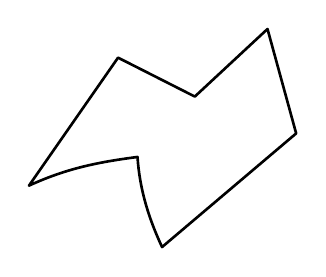
\begin{tikzpicture}[x=.013cm,y=-.013cm,line cap=round,line join=round]
  \draw[line width=.95pt] (274,1178)--(361,1053)--(436,1091)--(507,1025)
    --(535,1127)--(404,1238).. controls (390,1208) and (382,1180) ..(380,1150)
    .. controls (342,1155) and (311,1161) ..(274,1178)--cycle;
\end{tikzpicture}}
Si $\Gamma'=\partial E(\Gamma)$, où $\Gamma$ est un polygône (non convexe puisque $\Gamma'\ne\Gamma$), alors l'\deleted{\unsure{ens}} \inserted{$\unsure{\mathcal{L}|\mathscr{L}|L}$ des} extrémités des arcs polygonaux composantes connexes de $\Gamma\cap\Gamma'$ \deleted{sont des sommets de $\Gamma$} \inserted{\unsure{est|sont} $\subset S(\Gamma)$} \unsure{et pour|alors|pour} \unsure{toute|tout} \deleted{\unsure{tel|tels}} $s\in\mathcal{L}$, $\exists\,\deleted{\unsure{E}}t\in\mathcal{L}$, $t\ne s$, telle que $]s,t[\subset\Gamma'\deleted{\unsure{\operatorname{Ext}}}\cap\complement\Gamma$ et alors $]s,t[\subset\operatorname{Ext}\Gamma$.

% slanted
\margin{\uline{NB} $t$ est unique, sauf si $s$ point isolé de $\Gamma\cap\Gamma'$, auquel cas il existe \unsure{exactmt|exactem} deux tels $t$.}

\uline{Cor} Si $\Gamma$ polygône non convexe, $\exists\,s,s'$ sommets \unsure{distinct|distincts} de $\Gamma$, tel que $s$ \deleted{\unsure{et $s'$}, \unsure{visib} \unsure{de $s$}} $]s,s'[\subset\operatorname{Ext}\Gamma\cap\partial E(C)$

[\uline{NB} $\operatorname{Ext}(\Gamma)$ est défini pour \unsure{tt|ts} polygône, pas \unsure{néc.|néc} un \unsure{'|``}J-polygône\unsure{..|''} ]
% archive sheet number: 31
\scanpage{33}\mspage{VII}
\uline{Lemme} VII : Si $\Gamma$ est un J-polygone on a $\operatorname{ext}\partial E(\Gamma)\subset\operatorname{ext}\Gamma$.

\uline{Démonstration} : Comme $E(\Gamma)$ est un ensemble convexe $\operatorname{ext}\partial E(\Gamma)=\mathbb{R}^{2}-E(\Gamma)$ (d'aprés la preuve du lemme VI) donc $\operatorname{ext}\partial E(\Gamma)\cap\Gamma=\varnothing$ puisque $\Gamma\subset E(\Gamma)$.

Il est clair que $\operatorname{ext}\Gamma\cap\operatorname{ext}\partial E(\Gamma)\ne\varnothing$ (par exemple en prenant un triangle qui contient $R_{\Gamma}$ et $R_{\partial E(\Gamma)}$ à l'interieur on voit que l'exterieur est \unsure{comun|commun} à \deleted{\unsure{à|la}} $\operatorname{ext}\Gamma$ et a $\operatorname{ext}\partial E(\Gamma)$). Donc $\operatorname{ext}\partial E(\Gamma)\subset\operatorname{ext}\Gamma$ puisque $\operatorname{ext}\partial E(\Gamma)$ est connexe \inserted{et $\mathbb{R}^{2}-\Gamma=\operatorname{int}\Gamma\cup\operatorname{ext}\Gamma$.} cela prouve le lemme.

% slanted
\margin{\unsure{inutile|inutil}}
\uline{Lemme VII} : Si $\Gamma$ est un \inserted{(}J-\inserted{)}polygone non-convexe il existe $s,s'\in\mathbb{S}(\Gamma)$ tel que \deleted{\unsure{si}} $s'$ est visible de $s$ de l'exterieur de $\Gamma$.

\uline{Demonstration} : On sait que $\partial E(\Gamma)\cap\Gamma\ne\varnothing$ (puisque $\deleted{\unsure{\exists}}\partial E(\Gamma)\cap\Gamma\supset\mathbb{S}(\partial E(\Gamma))$) on veut montrer \inserted{que} $\partial E(\Gamma)\not\subset\Gamma$. Si $\partial E(\Gamma)\subset\Gamma$ alors \inserted{on prouve facilement que} $\partial E(\Gamma)$ est un sous-ensemble ouvert de $\Gamma$ et en plus fermé puisqu'il est compact donc $\partial E(\Gamma)=\Gamma$ en raison de la conexité de $\Gamma$, ce qui contredit le fait que $\Gamma$ est non-convexe.

% margin note written sideways
\margin{\deleted{\unsure{Compl.|Conclure|Concl.} \unsure{que} $\partial E(\Gamma)\subset\unsure{\Gamma}\ \unsure{\Rightarrow}\ \underset{\substack{\Vert\\ E(\Gamma)}}{E(\partial E(\Gamma))}\subset$ \unsure{bref}}}
Soit $\alpha$\inserted{$=[s,s']$} une arête de $\partial E(\Gamma)$ telleque $\alpha\not\subset\Gamma$. Si $]s,s'[\subset\mathbb{R}^{2}-\Gamma$ cela prouve le lemme puisque $s,s'\in\mathbb{S}(\Gamma)$.

Si $s$ est un point isolé de $\alpha\cap\Gamma$ Soit $t$ le point de $(\Gamma-s)\cap\alpha$ qui réalise la distance de $s$ a l'ensemble compact $\alpha\cap(\Gamma-s)=\alpha\cap\Gamma-\underbrace{\{s\}}_{\inserted{\text{ouvert dans }\alpha\cap\Gamma}}$. Il est clair par le choix de $t$ que $]s,t[\subset\mathbb{R}^{2}-\Gamma$. Prouvons que $t\in\mathbb{S}(\Gamma)$. Si $t\notin\mathbb{S}(\Gamma)$ il existe $\alpha'\in A(\Gamma)$ tel que $t\in$ au segment ouvert correspondant $=\mathring{\alpha}'$, mais alors comme $t\in\mathring{\alpha}'\cap\mathring{\alpha}$ on doit pouvoir trouver un ouvert $\subset\mathring{\alpha}'\cap\mathring{\alpha}$ \inserted{auquel $t$ appartient} cela contredit le choix de $t$, puisque $\mathring{\alpha}'\cap\mathring{\alpha}\subset\alpha\cap\Gamma$. Si $s$ n'est pas isolé on peut trouver une arête $[s,t_1]\in\unsure{A.|A}(\Gamma)$ telle que $[s,t_1]\subset\alpha$. Si $t_1$ est isolé on \unsure{réfait|réfoit} l'argument ci-dessus, dans le cas contraire on considère $[t_1,t_2]$-{}-etc. jusqu'à trouver $t$ isolé dans $[s,s']$.

Montrons maintenant que si $s,s'\in S(\Gamma)$ et $]s,s'[\subset\mathbb{R}^{2}-\Gamma$ si $[s,s']\subset\alpha\subset\partial E\unsure{[|(}\Gamma\unsure{]|)}$ $]s,s'[\subset\operatorname{ext}\Gamma$.
% archive sheet number: 32
\scanpage{34}\mspage{VIII}
Comme $]s,s'[\subset\mathbb{R}^{2}-\Gamma$ est connexe on a $]s,s'[\subset\operatorname{int}\Gamma$ ou bien $]s,s'[\subset\operatorname{ext}\Gamma$.

Si $t^{\deleted{\unsure{'|*}}}\in ]s,s'[$ alors $t\in\alpha\subset\partial E(\Gamma)$ \inserted{et \deleted{\illegible{1}} $t\in\mathbb{R}^{2}-\Gamma$,} Comme $\partial E(\Gamma)$ est un polygone convexe il vérifie la condition b) de la definition 1 (cf. lemme VI), on peut donc choisir $D_t\subset\mathbb{R}^{2}-\Gamma$ satisfaisant b). Mais $D_t\cap\operatorname{ext}\partial E(\Gamma)\ne\varnothing$ \inserted{donc $D_t\cap\operatorname{ext}\Gamma\ne\varnothing$ (cf lemme VII),} avec le fait que $D_t$ est connexe entraîne $D_t\subset\operatorname{ext}\deleted{\partial E(}\Gamma\deleted{)}$, donc $t\in\operatorname{ext}\deleted{\partial E(}\Gamma\deleted{)}$ ce qui prouve \inserted{que} $]s,s'[\deleted{\unsure{\subset}}\deleted{\mathbb{R}^{2}-E(\Gamma)\unsure{=|)|]}}\deleted{\operatorname{ext}\partial E(\Gamma)}\subset\operatorname{ext}\Gamma$, \deleted{en vertu du lemme VII}, c.q.f.d.

Si $\Gamma$ est un J-polygone et $s\in S(\Gamma)$, soit $D_s$ un disque de centre $s$ satisfaisant à b) de la def.\deleted{\unsure{2}}1, puisque $s$ appartient a deux arêtes de $\Gamma$ on a que $\Gamma\unsure{\Vert|\cap}D_s$ determine deux secteurs angulaires dont l'interieur de l'un est contenu dans $\operatorname{int}\Gamma$ (secteur interieur) et l'interieur de l'autre dans $\operatorname{ext}\Gamma$ (secteur exterieur).

\margin{$\unsure{\cdot|\bullet}$}
On a \deleted{donc} \inserted{alors} l'analogue suivant de la positivité de la courbure des courbes \inserted{de $\mathbb{R}^{2}$} convexes :

\uline{Lemme} IX : Si $\Gamma$ est un polygone convexe et $s\in\mathbb{S}(\Gamma)$ alors pour tout disque $D_s$ de centre $s$ qui satisfait b) de la def. 2 l'angle $\alpha$ qui ``sous tend'' le secteur circulaire interieur \unsure{vérifie|vérifié} $\alpha\le\pi$.

\uline{Demonstration} : Comme le secteur ang. interieur $=\overbrace{D_s}^{\inserted{\text{convexe}}}\cap\overbrace{\operatorname{int}\Gamma}^{\inserted{\text{convexe}}}$, on voit qu'il est convexe, mais un secteur angulaire est convexe si et seulement si son angle $\alpha$ vérifie $\alpha\le\pi$, c.q.f.d. .

\deleted{\unsure{Lemme} \illegible{3}}

\uline{Lemme X} : Si $\Gamma$ est un \deleted{J-}polygone il existe au moins trois sommets tels que pour tout disque $D_s$ qui satisfait b) \deleted{\illegible{1}}. de la def. 2 et de centre un de ces trois sommets l'angle du secteur angulaire interieur est inferieur à $\pi$.

\uline{Demonstration} : Soit $s\in\mathbb{S}(\partial E(\Gamma))\subset S(\Gamma)$ et soient $s',s''$ les deux sommets de $\partial E(\Gamma)$ qui sont consecutifs à $s$. Le lemme II nous dit que $s,s',s''$ ne sont pas colineaires.
% archive sheet number: 33
